\section{Threads}
Partiamo con il distinguere un thread da un processo. Il thread è un \textbf{filo di esecuzione}: in un processo ci possono essere diversi thread i quali possono avere dei diversi \textit{pattern} per ciascuna esecuzione.

\subsubsection*{Perché?}
I thread sono entità più semplici rispetto ai processi e sono quindi più facili da gestire. Grazie ai thread si ottengono diversi vantaggi:
\vspace{-5px}
\begin{itemize}
\setlength{\itemsep}{-.25 em}
    \item Il sistema è più \textbf{recettivo};
    \item Dato che le risorse sono condivise è più facile gestirle;
    \item Richiede meno risorse rispetto alla creazione di un processo;
    \item Può utilizzare tutti i \textit{core} messi a disposizione dal sistema (\textit{multicore programming}).
\end{itemize}

\noindent Per esempio, al posto di far eseguire 4 processi differenti è molto meglio eseguire un processo con 4 thread differenti: in questo modo si evita di allocare in memoria 4 volte le stesse risorse che, grazie all'utilizzo dei thread, sono allocate solo una volta. 
% 
\subsection{Concorrenza e parallelismo} \label{parallelismo}
Quando parliamo di \textbf{multicore programming} è necessario fare una netta distinzione tra il significato di concorrenza e parallelismo. Con \textbf{parallelismo} si intende che un sistema è in grado di preformare più di un compito in maniera simultanea (tipico dei sistemi multicore). Con \textbf{concorrenza} si intende la possibilità di far progredire più di un compito (non in maniera simultanea).

Come possiamo vedere della figura \ref{fig:concorrenza}, quando parliamo di concorrenza ci riferiamo ad un singolo core che esegue a frammenti più thread diversi.
\begin{figure}[!h]
    \centering
    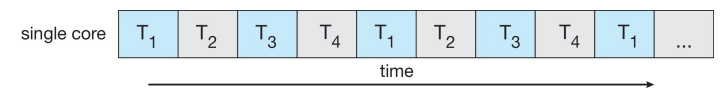
\includegraphics[width=.7\textwidth]{../res/imgs/threads/concorrenza.png}
    \caption{Esempio di concorrenza tra 4 processi.}
    \label{fig:concorrenza}
\end{figure}

Quando invece facciamo riferimento al parallelismo (figura \ref{fig:parallelismo}) indichiamo la capacità del sistema di effettivamente riuscire ad eseguire parallelamente diversi thread. 
\begin{figure}[!h]
    \centering
    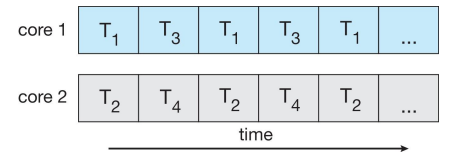
\includegraphics[width=.5\textwidth]{../res/imgs/threads/parallelismo.png}
    \caption{Esempio di parallelismo in un sistema dual core.}
    \label{fig:parallelismo}
\end{figure}
Si osserva che le due pratiche non sono esclusive: notiamo che il core 1 esegue in maniera concorrente T1 e T3, mentre il core 2 esegue in maniera concorrente T2 e T4.

\subsubsection{Tipi di parallelismo}
Possiamo dividere i parallelismi in due tipi. Il primo, chiamato \textbf{data parallelism} (figura \ref{fig:data_parallelism}) implica un sottoinsieme preciso di dati sia distribuito per ogni core. In altre parole, avendo a che fare un un largo database, lo si suddivide in parti e ciascuna viene assegnata ad un core. Tale core potrà operare solo in quella porzione di dati
\begin{figure}[!h]
    \centering
    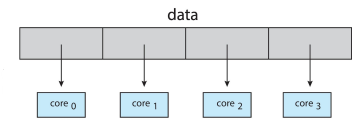
\includegraphics[width = .5\textwidth]{../res/imgs/threads/data_parallelism.png}
    \caption{Esempio di parallelismo di dati.}
    \label{fig:data_parallelism}
\end{figure}

\noindent Il secondo tipo di parallelismo è detto \textbf{task parallelism}, rappresentato in figura \ref{fig:task_parallelism}. Questo tipo di parallelismo concede la memoria condivisa a ciascun core solo che ogni core ha un compito ben preciso: un core sarà ottimizzato per la scrittura, un altro sarà più veloce in lettura e così via.
\begin{figure}[!h]
    \centering
    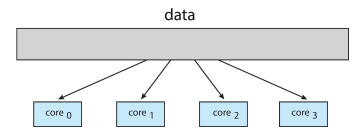
\includegraphics[width=.5\textwidth]{../res/imgs/threads/task_parallelism.png}
    \caption{Esempio di parallelismo di compiti.}
    \label{fig:task_parallelism}
\end{figure}
% 
\subsubsection{Legge di \textit{Amdahl}}
La legge di \textit{Amdahl} è una funzione che mette in relazione due variabili importanti:
\vspace{-5px}
\begin{enumerate}
\setlength{\itemsep}{-.15 em}
    \item \textbf{S}, ovvero la percentuale di codice che non può essere parallelizzato, ovvero codice \textbf{seriale} (di conseguenza il numero di codice che può essere parallelizzato è $1 - S$);
    \item \textbf{N}, che rappresenta il numero di core disponibili. 
\end{enumerate}

\noindent Con questi due dati abbiamo la possibili di calcolare lo \textit{\textbf{speedup}} attraverso la seguente formula:
\begin{equation*}
    \text{\textit{speedup}} \leq \frac{1}{S + \frac{1 - S}{N}}
\end{equation*}

\noindent Osservando la formula osserviamo che se se la percentuale di codice seriale tende a zero e il numero di core tende a infinito, lo \textit{speedup} sarebbe infinito. Questa però è una situazione utopica: non esistono casi in cui si è privi di codice seriale.

Osserviamo quindi il seguente grafico (figura \ref{fig:speedup}) che mostra lo \textit{speedup} all'aumentare del numero di core, essendo a conoscenza della percentuale di codice seriale.
\begin{figure}[!h]
    \centering
    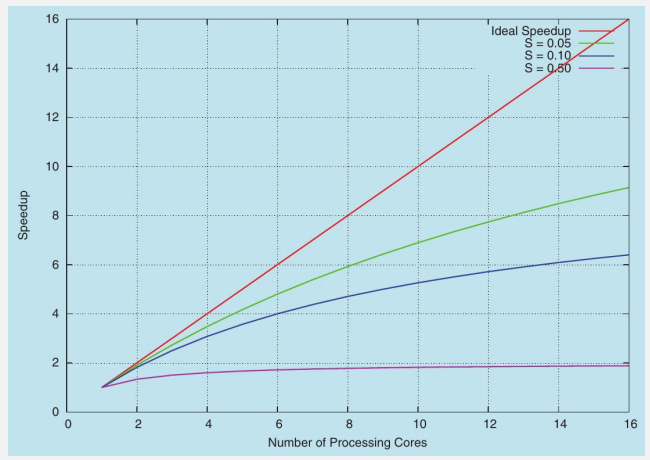
\includegraphics[width=.6\textwidth]{../res/imgs/threads/speedup.png}
    \caption{Il grafico che descrive lo \textit{speedup} a seconda della percentuale di codice seriale.}
    \label{fig:speedup}
\end{figure}
Notiamo che quando la percentuale di codice seriale è circa la metà non ha importanza il numero di core del sistema: lo speedup rimarrà pressoché invariato. Anche solo con il 5\% di codice seriale notiamo un forte abbassamento rispetto allo speedup ideale. È evidente quindi che l'aumento di core non causa l'aumento di speedup, sopratutto in una situazione dove il codice seriale è molto. 
% 
\subsection{Modelli multithreading}
È importante fare una distinzione tra due classi principali di thread: \textbf{user threads} e \textbf{kernel threads}. La principale differenza tra i due è che i kernell threads hanno molti più privilegi rispetto a quelli utente. Esistono quindi dei modelli che cercano di associare agli user threads i kernell threads al fine di sfruttare al meglio il principio di \textit{multithreading}.

\subsubsection{Many-to-One}
In questa prima architettura, il kernell mette a disposizione solo un thread che è collegato e deve soddisfare tutte le richieste di tutti gli user threads (figura \ref{fig:many_to_one}).
\begin{figure}[!h]
    \centering
    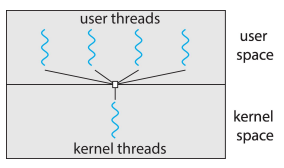
\includegraphics[width = .5\textwidth]{../res/imgs/threads/many_to_one.png}
    \caption{Il modello di \textit{multithreading} molti a uno.}
    \label{fig:many_to_one}
\end{figure}
È evidente che l'efficienza di questo modello non è il suo forte: sono presenti diversi thread utente ai quali deve rispondere solamente un thread del kernel. Basta pesare al fatto che se il kernel thread è in attesa di un input esterno, tutti gli user thread sono bloccati (\textbf{collo di bottiglia}). Questo modello è infatti poco utilizzato dato che non sfrutta le potenzialità del \textit{multicore}. 
% 
\subsubsection{One-to-One}
In questa architettura (figura \ref{fig:one_to_one}), quando viene creato uno user thread, il suo rispettivo kernel thread viene creato; così facendo esiste un kernell thread associato ad ogni user thread. 
\begin{figure}[!h]
    \centering
    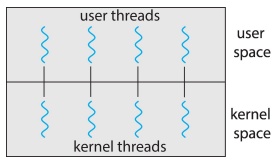
\includegraphics[width = .5\textwidth]{../res/imgs/threads/one_to_one.png}
    \caption{Il modello di \textit{multithreading} uno a uno.}
    \label{fig:one_to_one}
\end{figure}
Ad ogni modo ci possono essere alcune restrizioni in modo da evitare la creazioni di troppi kernel threads (e quindi limitare la creazione di user threads). È comunque evidente che questo modello è sicuramente più \textbf{efficace} del modello precedente in quanto fornisce la possibilità di sfruttare a piano un sistema multicore.
% 
\subsubsection{Many-to-Many}
L'ultimo modello è un buon compromesso tra il modello \textit{Many-to-One} e il modello \textit{One-to-One}. Il modello molti a molti (figura \ref{fig:many_to_many}) fornisce diversi vantaggi ed è più flessibile rispetto ai primi due. Non esiste infatti la corrispondenza univoca, generalmente si hanno più user threads che fanno riferimento ad alcuni kernell threads (è come se una sala da 20 clienti fosse gestita da 5 camerieri). 
\begin{figure}[!h]
    \centering
    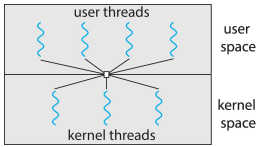
\includegraphics[width = .5\textwidth]{../res/imgs/threads/many_to_many.png}
    \caption{Il modello di \textit{multithreading} molti a molti.}
    \label{fig:many_to_many}
\end{figure}
È possibile infatti controllare in maniera più efficace i kernell thread e questo rende il modello \textit{Many-to-Many} molto \textbf{robusto}. Ad ogni modo la sua implementazione è molto più complessa rispetto ai modelli precedenti.

Per questo, a volte, si fa riferimento ad un \textit{ibrido} tra il modello \textit{Many-to-Many} e il modello \textit{One-to-One}: stiamo parlando del \textbf{Two-level model} che consente sia la corrispondenza \textit{1 a 1} che la corrispondenza \textit{N a M}.

% 
\subsection{Librerie di thread}
In questa piccola sezione ci interessiamo alle libreire disponibili per la creazione e la gestione di threads. Queste possono essere di due tipi:
\begin{itemize}
\setlength{\itemsep}{-.15 em}
    \item Librerie in \textbf{user space}, dove i thread sono gestiti completamente a livello utente (come nel caso di \texttt{Pthreads});
    \item Librerie di tipo \textbf{kernel-level} che sono supportate dal sistema operativo e si appoggiano al kernel attraverso le \textit{system calls}; questo comporta un livello maggiore di complessità nel kernell ma il programmatore ha meno da implementare.
\end{itemize}

\noindent Spendiamo due parole su \texttt{POSIX Threads}. Questa, non è propriamente una libreria ma è un insieme di specifiche (non implementazioni!) che aiuta con la creazione e la gestione di thread. \texttt{POSIX Threads} fornisce specifiche sia a livello di utente che a livello di kernel.

% 
\subsection{Threading implicito}
Cerchiamo ora di cambiare approccio: attraverso le librerie l'approccio era esplicito, stava al programmatore l'implementazione e/o la gestione dei thread. Nel momento in cui si fa riferimento a più threads, diventa sempre più difficile controllare la correttezza del codice. Ecco che si è pensato ad un altro approccio: il threading \textbf{implicito}. Con questo approccio i thread sono gestiti maggiormente dal compilatore oppure da librerie \textit{run-time} le quali si occupano di creare e gestire i thread. In questa sezione vedremo alcuni dei metodi utilizzati per ottenere il threading implicito. 
% 
\subsubsection{Modello fork-join}
Questo tipo di modello si ispira alla creazione di processi (paragrafo \ref{creazione di un processo}). In questo modello, diversi threads sono divisi e, una volta che sono terminati, vengono uniti (figura \ref{fig:fork_join}). La divisione dei threads è una scelta presa completamente dalla libreria.
\begin{figure}
    \centering
    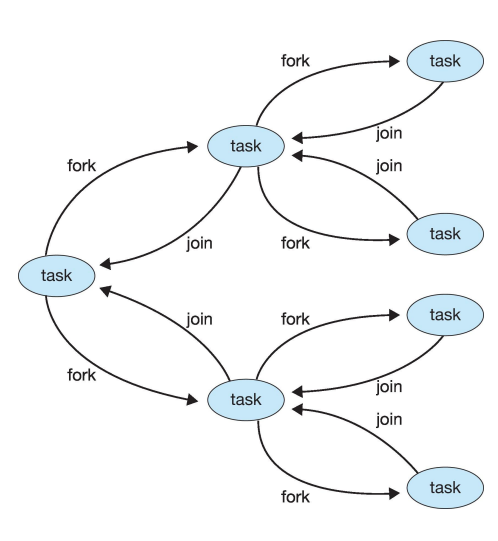
\includegraphics[width = .4\textwidth]{../res/imgs/threads/fork_join.png}
    \caption{Rappresentazione grafica del modello fork-join per la risoluzione di un task.}
    \label{fig:fork_join}
\end{figure}
Come possiamo notare dalla figura \ref{fig:fork_join}, in questo caso, la libreria sceglie un task da far risolvere ad un thread dove, eventualmente verrà splittata in altri due thread (che vengono appositamente creati) e così via fino a che il task non sia completamente risolto.
% 
\subsubsection{Thread pools e OpenMP}
Altri due modelli molto importanti sono \textit{thread pools} e \texttt{OpenMP}. Nel primo caso la libreria mette a disposizione un numero di thread (\textit{pool} di thread) che attendono un  task da risolvere. In questo modo, dato che i thread sono già pronti, non si spreca tempo per l'effettivo processo di creazione. Inoltre il problema della limitazione dei thread è risolto in quanto una volta creati quelli per la \textit{pool}, non vengono creati altri thread. 

Quando parliamo di \texttt{OpenMP} invece parliamo di una serie di \textbf{direttive} per il compilatore e un insieme di librerie per \texttt{C}, \texttt{C++} e \texttt{FORTRAN}. Questo modello fornisce tutte le risorse per la condivisione della memoria tra i thread e i parallelismi. Essendo delle direttive, queste devo essere proprio scritte nel codice; per esempio: \texttt{\#pragm omp parallel}.
% 
\subsection{Problematiche}
Come vedremo in questo paragrafo, anche i thread portano a delle problematiche che devono essere gestite come, per esempio, l'interruzione di tali e il modo di implementare l'eliminazione di un thread.

\subsubsection{Semantica \texttt{exec} e \texttt{fork}}
Il primo dubbio che è necessario chiarire è il comportamento durante la chiamata della funzione \texttt{exec()}: se si fa una chiamata alla funzione \texttt{exec()}, vengono rimpiazzati tutti i thread del processo oppure solo il thread su cui è stata chiamata \texttt{exec}? Generalmente la funzione \texttt{exec} cancella il processo in esecuzione e, di conseguenza, tutti i sui thread.

Il secondo dubbio, riguarda la funzione \texttt{fork()}: se si fa una chiamata a \texttt{fork()} ad un processo multithread, si effettua una copia a tutti i thread del processo oppure solo al thread su cui è stata chiama la funzione? La risposta a questa domanda è che dipende dall'obiettivo della funzione \texttt{fork()}:
\vspace{-5px}
\begin{itemize}
\setlength{\itemsep}{-.15 em}
    \item Se la funzione deve cambiare subito il codice attraverso \texttt{exec()}, non vale la piena copiare tutti i thread se tanto si si che verranno eliminati.
    \item Se invece il nuovo processo deve supportare anch'esso il multithreading, allora ha senso effettuare una coppia di tutti i thread e non solo del thread su cui è stata chiamata la funzione
\end{itemize}
% 
\subsubsection{Segnalazione ed eliminazione}
I segnali sono usati per notificare un processo che un determinato evento è accaduto. Tali segnali però debbono essere gestiti: ecco che emerge la figura del \textbf{signal handler} che può essere di \textbf{default} oppure \textbf{user-defined}, ovvero definito dall'utente. Generalmente ogni segnale ha il suo specifico \textit{default handler} che è utilizzato anche dal kernel. Cosa succede però nel caso in cui il sistema è multi-threading? Ci sono diverse opzioni:
\vspace{-5px}
\begin{enumerate}
\setlength{\itemsep}{-.15 em}
    \item Spedire il segnale al thread ad esso compatibile;
    \item Propagare il segnale ad ogni thread del processo;
    \item Mandare il segnale ad dei thread specifici del processo;
    \item Assegnare ad uno specifico thread il compito di ricevere i segnali degli altri thread.
\end{enumerate}

\noindentÈ inoltre importante riuscire a gestire la \textbf{cancellazione} dei thread. Questi però devono attivare la possibilità di essere cancellati: in altre parole, se un thread ha la cancellazione disabilitata non potrà essere cancellato fino a che non viene riattivata. Nel momento in cui la cancellazione è attivata, il thread può essere cancellato attraverso due tecniche:
\vspace{-5px}
\begin{itemize}
\setlength{\itemsep}{-.15 em}
    \item \textbf{Asincrona}, ovvero il thread termina immediatamente;
    \item \textbf{Deferred} che significa \textit{posticipata}. Può ritornare utile nel momento in cui il thread sta compiendo un'operazione delicata (chiusura di un file) e non ha la possibilità di terminare immediatamente. 
\end{itemize}


